\chapter{Konzeption}
\label{cha:konzeption}
Bei der Konzeption wurde der aktuelle Stand des bestehenden Webauftritts betrachtet und analysiert. Im weiteren Schritt wurden Erweiterungen für die Website geplant. Im nächsten großen Schritt erfolgte eine Analyse aktuell bestehender Software, welche Gegenstände verwaltet.


\section{Analyse des aktuellen Webauftritts}
\label{webauftritt}
Der Webauftritt, erreichbar im Netzwerk der Hochschule Furtwangen\url{http://web.smarthome.hs-furtwangen.de/}, des \ac{SHL} Labors, wird mit der Hilfe des \ac{CMS} WordPress verwaltet. WordPress eigne sich hier, weil es mittels \ac{UX} so gestaltet wurde, das es sehr leicht zu erlernen ist. Unerfahrene Benutzer könne so schnell eigene Inhalte einpflegen.

\begin{figure}[bh]
	\centering
	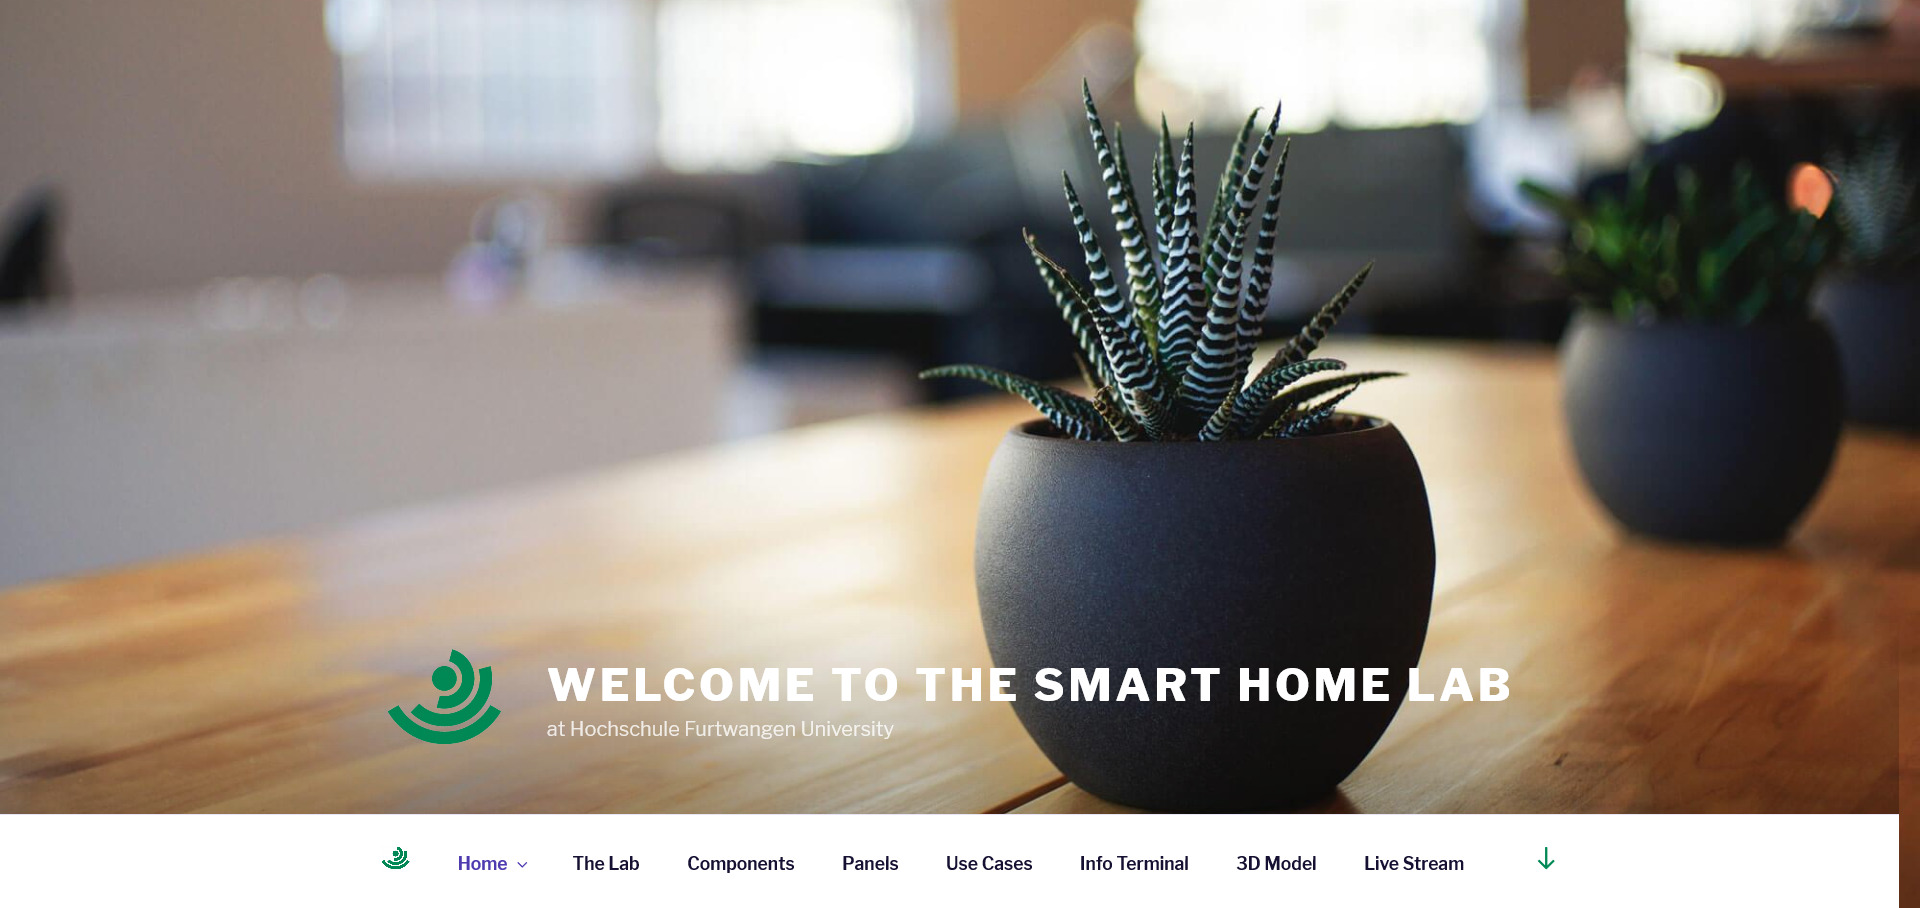
\includegraphics[scale=0.23]{content/pictures/shlwebsit.jpg}
	% bosch_iot_poll.png: 0x0 pixel, 300dpi, 0.00x0.00 cm, bb=
	\caption{Die Startseite des Webauftritts}
	\label{fig:web}
\end{figure}

Die Website ist mit dem, von WordPress eigenem Designe Twentyseventeen gestaltet. Auf der Startseite sieh man ein großes Headerbild. Darunter Folgt eine Navigationsleiste, welche die Links bei einem Besuch einer Unterseite in einem Lila Farbton darstellt. Die Navigation umfasst die Seiten:

\begin{itemize}
	\item Home
	
	\item The Lab 
	
	\item Components 
	
	\item Panels
	
	\item Use Cases 
	
	\item Info Terminal
	
	\item 3D Model
	
	\item Live Stream
	
	
	
\end{itemize}

Weiter folgt eine kurze Beschreibung über das Labor. Der nächste Abschnitt der Startseite stellt das Team vor. Im Anschluss sieht man noch ein Video, welches das Labor vorstellt, ein Kontaktforumlar und die Addresse mit einer Google Maps Karte. Am untersten Ende ist ein Footer, welche eine Copyright und einen Link zum Impressum enthält.

Die Unterseite \glqq The Lab\grqq stellt das Labor mit Grundrissen etwas detailreicher vor. \glqq Components\grqq stellt wenige, aber wichtige Geräte vor. In \glqq Panels\grqq werden, die mit Sensoren und Geräte versehenen, Wände in den Räumen beschrieben. Eine Auswahl von umgesetzten Anwendungsfällen werden in der Unterseite \glqq Use Cases\grqq beschrieben. Für das Infoterminal gibt es ebenfalls eine Unterseite, welche automatisiert eine Präsentation über das Labor abspielt. Unter dem Punkt \glqq 3D Model\grqq, befindet sich eine 3D Ansicht des Labors, welches sich in einer Ego- und Vogelperspektive betrachten lässt. Auch können hier vereinzelt Geräte bedient werden. Abgeschlossen wird die Navigation mit einer Unterseite, welche einen Video Livestream zeigen kann.

 

\subsection{Corporate Design}
Mit den aktuellen Farben entspricht der Webauftritt des Labors nicht dem \ac{CD} der Hochschule Furtwangen. So müssen die Lila Farben durch die Farbe Grün mit dem Hexwert 83b62d geändert werden. Dies ist wichtig um einen Wiedererkennungswert der Hochschule darzustellen. Die Navigation stellte hier einen größeren Bruch dar. Um die Seite vollständig im \ac{CD} der Hochschule zu haben, ist ein Expertengespräch nötig.



\subsection{Erweiterung des Webauftritts}
Neben dem \acf{CD} gab es noch weitere Punkte, welche den Auftritt noch Informativer und attraktiver gestalten konnten. So stehen im Labor die einzelnen Räume: Küche, Bad, Multimediaraum, IoT-Raum und der Arbeitsbereich stark im Vordergrund. Diese wurden bisher nur sehr dürftig auf der Homepage erwähnt. Daher wurde für die Räume eigene Unterseiten angelegt. Um auf \acf{UX} zu achten, wurde mittels des WordPress-Plugin Draw Attention  eine Interaktive Karte erzeugt. Bei einem Klick auf einen Raum, erhält der User mehr Informationen. \autocite{WPDrawAttention.}

\begin{figure}[H]
	\centering
	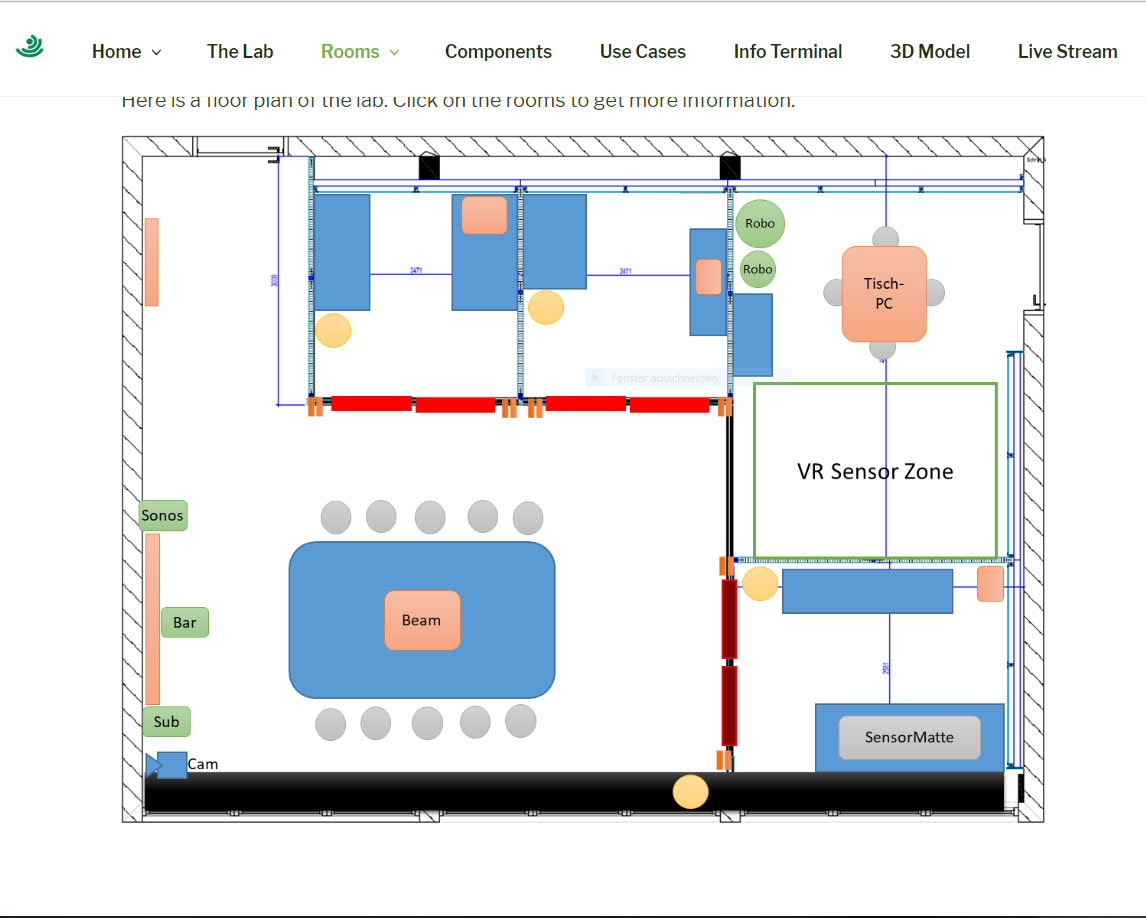
\includegraphics[scale=0.35]{content/pictures/room.jpg}
	% bosch_iot_poll.png: 0x0 pixel, 300dpi, 0.00x0.00 cm, bb=
	\caption{Raumkarte}
	\label{fig:room}
\end{figure}

Jeder Raum hat seine eigene Unterseite, welche die Aufgaben des Raumes und dessen Ausstattung beschreibt.
\newpage
Die Netzwerkarchitektur im Labor ist sehr komplex. Wenn man nicht gerade mit am Aufbau dieser Architektur gearbeitet hat, kann schnell der Überblick verloren werden. Eine Übersichtskarte (siehe Abbildung \ref{fig:network}), auf welcher man sieht wo sich Server, Router und Gateways befinden, kann helfen um herauszufinden, wo bei Problemen mal nachgesehen werden kann. Diese findet man in der Navigation unter dem neuen Punkt Räume. Neben der Karte gibt es zu jedem Raum eine eigene Unterseite, wo auf dessen Netzwerkeigenschaften genauer eingegangen wird. Die Karte wurde mit Adobe Illustrator CC 2017 erzeugt. Dabei wurde, um die Übersichtlichkeit nicht zu gefährden, sehr auf Schlichtheit geachtet. Nur das nötigste wurde eingezeichnet. Neben der Einfachheit halten sich die Farben Grün und Weiß an das \ac{CD} der Hochschule Furtwangen.

\begin{figure}[H]
	\centering
	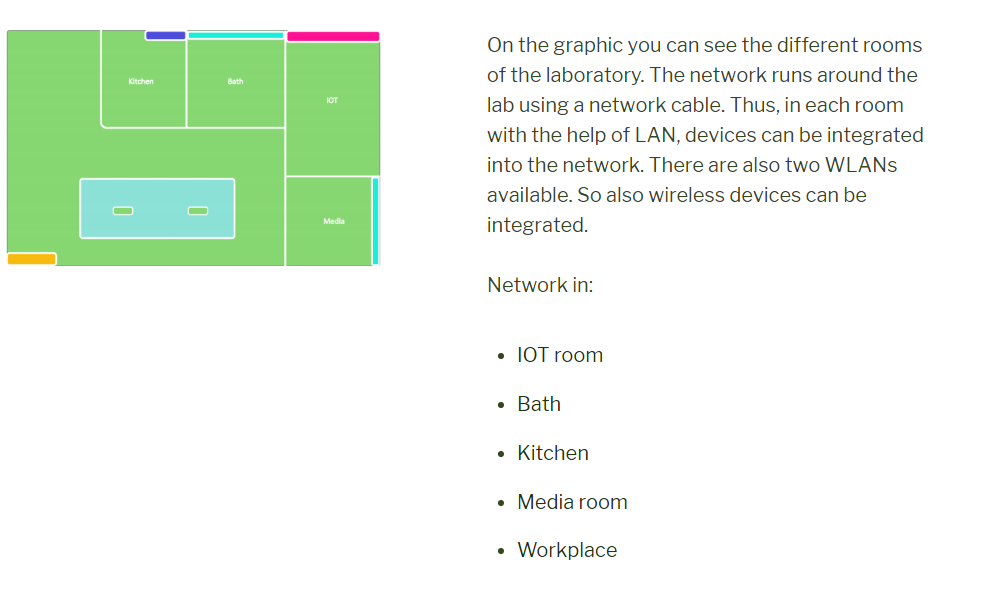
\includegraphics[scale=0.35]{content/pictures/network.png}
	% bosch_iot_poll.png: 0x0 pixel, 300dpi, 0.00x0.00 cm, bb=
	\caption{Netzwerkkarte}
	\label{fig:network}
\end{figure}

\section{Konzeption des Inventarisierungssystem}
\label{konzept:inventar}
Das Inventarisierungssystem ist das Herzstück dieser Masterthesis. Mit ihm können alle Gegenstände verwaltet werden und dazu noch sehr einfach und übersichtlich. Dabei spielt \acf{UX} und damit auch das \acf{UI} eine sehr große Rolle. Um einen Überblick zu bekommen was der aktuelle Markt zu bieten hat, müssen Vergleichbare Verwaltungssysteme(siehe Kapitel \ref{konzept:vergleich}) analysiert werden. Damit eine reibungslose Programmierung erfolgen kann müssen Konzepte für die Architektur der Anwendung ausgearbeitet werden.


\section{Vergleichbare Inventarisierungssysteme}
\label{konzept:vergleich}

Sucht man nach Inventarisierungssysteme stößt man immer wieder auf Software für Webshops. Mit ihnen hat man sehr häufig einen riesigen Umfang an Funktionen, mit welchen man nicht nur sein Inventar, sondern auch seine Verkäufe Verwalten kann.

\subsection{Magento}
\label{konzeption:magento}
Magento\footnote{https://magento.com} ist eine Openen-Source-E-Commerce Plattform und steht unter der Open Software License\footnote{https://opensource.org/licenses/osl-3.0.php}. Umgesetzt wurde es mit dem \acp{PHP} Framework Zend und lässt sich durch zahlreiche Plug-Ins erweitern.\autocite{.2018}

\begin{figure}[H]
	\centering
	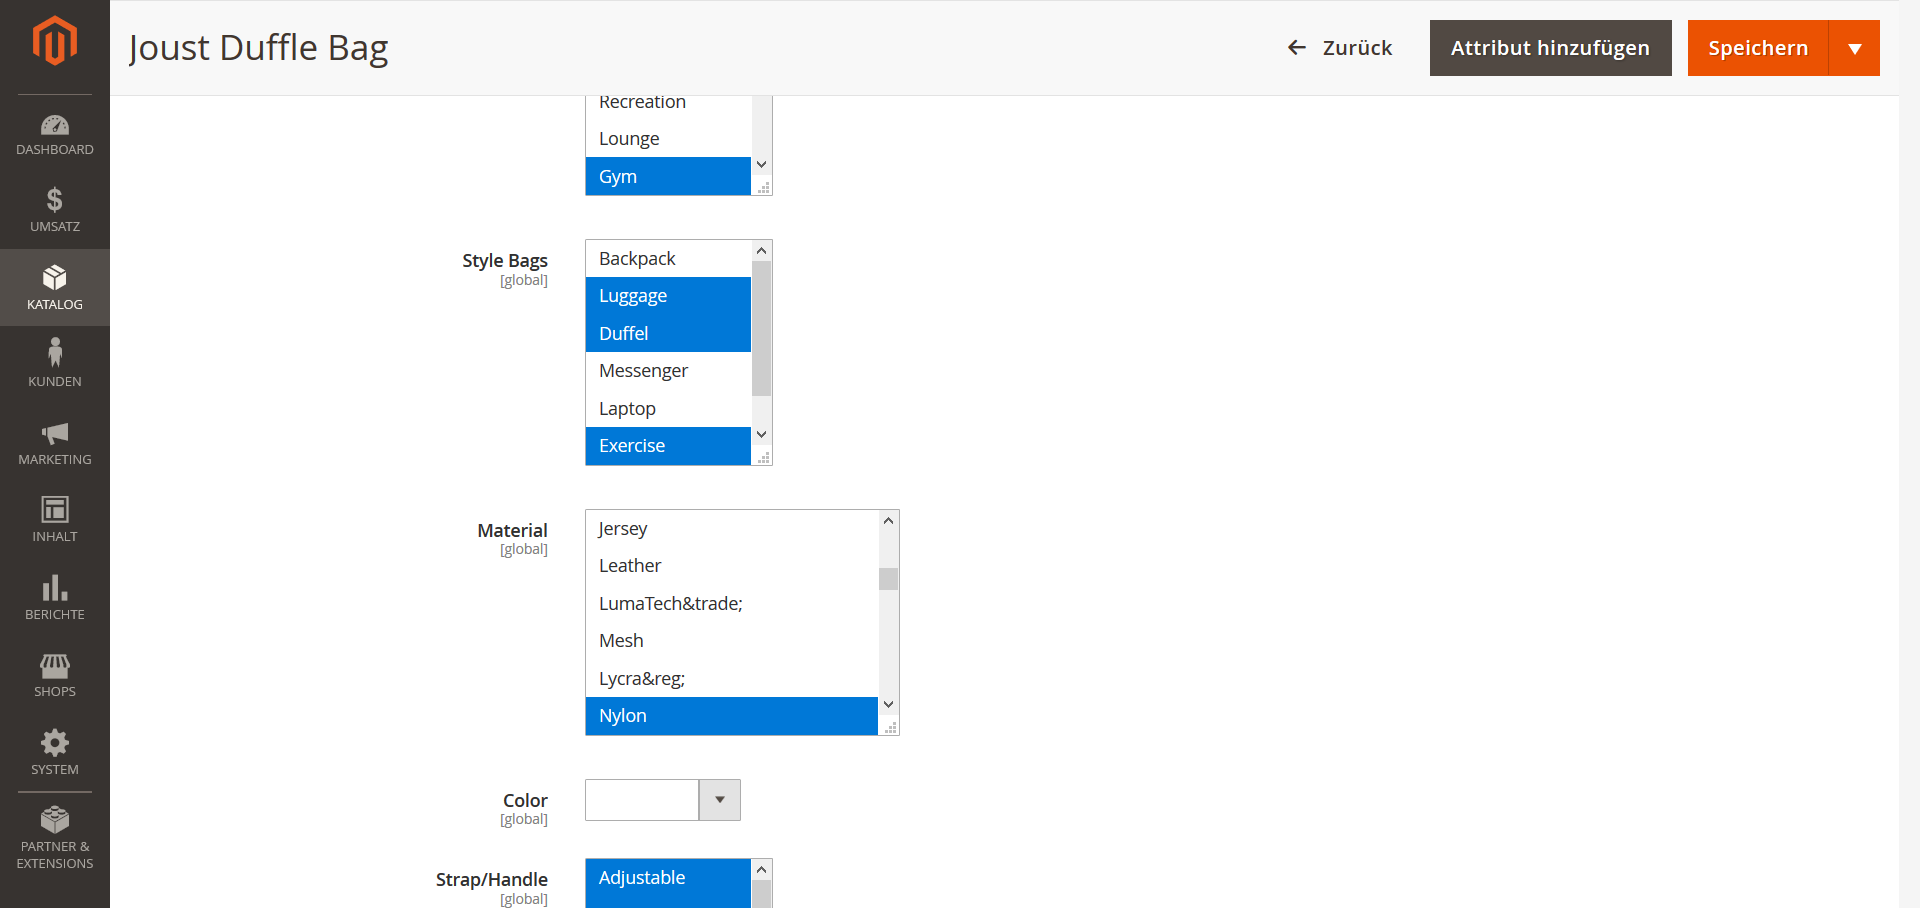
\includegraphics[scale=0.35]{content/pictures/magento.png}
	% bosch_iot_poll.png: 0x0 pixel, 300dpi, 0.00x0.00 cm, bb=
	\caption{Magento Itemverwaltung}
	\label{fig:magento}
\end{figure}

\subsubsection{Vorteile von Magento}
Magento bringt zahlreiche Verwaltungsoptionen. Man kann bis in das kleinste Detail einen Webshop konfigurieren und verwalten. Eine Rollenverteilung der User wird ebenfalls geboten. Jeder Gegenstand kann mit vorgefertigten und eigen angelegten Eigenschaften versehen werden. Das \ac{UI} von Magento ist ähnlich wie bei WordPress sehr benutzerfreundlich. Mit ein wenig Erfahrung findet man sich schnell zurecht. \autocite{Koch.2012}

\subsubsection{Nachteile von Magento}
In seiner größe, liegt der Nachteil des Frameworks. Es bietet zu viele Funktionen, welche nicht für ein Inventursystem in einer Laborumgebung benötigt werden. Damit belegt es unnötig Speicherplatz und lädt Dateien, welche nicht gebraucht werden. Auch wenn die Lernkurve sehr flach ist, muss eine gewisse Einarbeitung doch erfolgen. Auch ist mit der aktuellen Version von Magento eine Aktualisierung der \ac{PHP} Version nötig. \autocite{Koch.2012}

\subsection{WooComerce}
Anders als bei Magento (siehe Kapitel \ref{konzeption:magento}) steht das WordPress-Plugin, welches auch als E-Commerce Software dient unter der \ac{GNU} Lizenz. 

\subsubsection{Vorteile von WooComerce}
Bei Kostenlose WordPress-Plugin ist kostenlos und sehr einfach zu installieren. Mit einem klick ist es aus dem Plugin Bereich gewählt und kann mit einem Installationsassistenten den eigenen Bedürfnissen nach angepasst werden. Ein erfahrener WordPress-Nutzer hat eine deutlich niedrigere Lernkurve, als bei Magento \autocite{WooComerce.2018}

\subsubsection{Nachteile von WooComerce}
Die Nachteile sind ähnlich wie bei Magento. Es beinhaltet zu viele Funktionen, welche nicht gebraucht werden. Außerdem ist es sehr schwer möglich es nicht als Webshop, sondern als Verwaltungssystem zu nutzen. WooComerce gibt hier sehr starke richtlienen vor. So muss man schon im Installationsassisten sich gedanken über Maße, Bezahlmethoden und Versand machen. Was für ein Inventarisierungssystem nicht nötig ist. Mit WComerce ist man stark an WordPress gebunden. Solle man das \ac{CMS} wechseln wollen, ist ein mitnehmen der Anwendung nicht möglich.

\subsection{Entscheidung zur eigenen Anwendung}
Die Entscheidung eine eigene Anwendung zu schreiben wurde schon früh getroffen. Es muss eine Anwendung zur Verfügung gestellt werden, welche nicht mit Funktionen überladen ist. Die Lernkurve muss für jeden Anwender möglichst flach gehalten sein. Der Aufwand Magento oder WooComerce in das Hochschul \ac{CD} zu bringen, kann ein großer Aufwand sein. Daher lohnt es sich die Anwendung selbst zu schreiben. So bleibt sie Konfigurierbar und es werden nur \ac{PHP} Kenntnisse und keine spezielen WordPress oder Magento-Kenntnisse vorausgesetzt. Bei einem Wechsel zu einem anderen \ac{CMS} kann die Anwendung ebenfalls übernommen werden.

\section{Anforderungen}

Mit dem Anforderungsmanagement werden mögliche Features definiert. In der Anforderungsanalyse werden Eigenschaften, Funktionalitäten und die Qualität an die Software Festgehalten. \autocite{Grande.2014} Es werden funktionale und nicht-funktionale Anforderungen niedergeschrieben. Mit diesen Anforderung entsteht eine Definition und Ziele an die Anwendung.

\begin{itemize}
	\item Das Inventarisierungssystem muss alle Items in einer Laborumgebung aufnehmen. 
	
	\item Dabei soll bekannt sein wie der aktuelle Zustand der jeweiligen Items ist. 
	
	\item Die Datenbank sollen durchsuchbar sein. 
	
	\item Es müssen neue Items angelegt und alte gelöscht werden können. 
	
	\item Es soll für jeden Benutzer einen persönlichen Bereich geben. 
	
	\item Es soll Verschiedene Rollen für die Administration und User geben.
	
	\item Jeder Benutzer muss seine Persönlichen Daten verändern können.
	
	\item Benutzer können über den Administrator oder einem dazu befugten Mitarbeiter Items leihen.
	
	\item Benutzer sollen an die Rückgabe der geliehenen Items erinnert werden.
	
	
\end{itemize}

Ist eine solche Liste von Anforderungen erstellt worden, erhält man eine gute Übersicht über die zu entwickelnden Teilbereiche.

\newpage


\section{Datenbank}
\label{konzept:database}

\begin{figure}[bh]
	\centering
	\includegraphics[scale=0.35]{content/pictures/inventarER.png}
	% bosch_iot_poll.png: 0x0 pixel, 300dpi, 0.00x0.00 cm, bb=
	\caption{ER-Diagramm}
	\label{fig:erdiagram}
\end{figure}

Mit der Idee der Webanwendung, wurde schon sehr früh mittels einer Mindmap jede mögliche Eigenschaften aufgeschrieben. Aus dieser Mindmap konnte sehr komfortabel ein ER-Diagramm erzeugt. Um Redundanzen zu vermeiden, muss eine Normalisierung durchgeführt werden. In der Regel sind Redundanzen mit den ersten drei Normalformen abgeschlossen. Im ersten Schritt wurde darauf geachtet, das alle Eigenschaften Atomar sind. Vorname, in der Datenbank firstname und Nachname, in der Datenbank lastname, müssen als einzelne Eigenschaften zur Verfügung stehen. Eine Eigenschaft, mit dem Namen fullname, ist nach der ersten Normalform nicht erlaubt. Um die zweite Normalform zu erfüllen, muss die erste Normalform erfüllt sein und jedes Nichtschlüsselattribut von jedem Schlüsselkandidaten voll funktional abhängig sein. So wird festgestellt welche Eigenschaften eindeutig sind. Das ist nicht immer möglich, wie auch im Fall der Items Tabelle. Jeder Barcode in der Items-Tabelle ist einzigartig, jedoch gibt es Produkte, welche bewusst keinen Barcode haben. Gelöst wurde das Problem mit dem Künstlichen Primärschlüssel ID.\autocite{DatenbankenVerstehen.2018b} Die höchste Priorität der Normalsierung ist das vermeiden von Redundanzen und kann nur mit der 3. Nomalform erreicht werden.  Hierfür wurde die Hilfstabelle Lending eingefügt. Feststellen kann man das, in dem man überprüft, ob es viele-zu-viele existieren. Denn ohne diese Tabelle käme es zu Problemen, wenn sich eine Person mehrere Items leihen möchte.\autocite{DatenbankenVerstehen.2018}


\section{MockUps}
Um die geplante Idee umzusetzen ist es nötig ein MockUp zu erstellen. Doch bevor das MockUp erstellt werden kann, muss Storytelling betrieben werden. Beim Storytelling werden. Beim Storytelling geht es um Geschichten erzählen. Dabei werden die Anforderungen in realistische kleine Geschichten erzählt. So wird es leichter sich vorzustellen, wie ein Programm funktioniert. Diese Geschichten werden sachlich aufgeschrieben. An diesen Geschichten kann früh festgestellt werden, ob sich eine Idee nicht oder nur sehr aufwändig umsetzen lässt. Hier tritt auch die \acl{UX} in den Vordergrund, da man sich beim Schreiben in den User hineinversetzen muss. \autocite{Schach.2017}


\begin{figure}[bh]
	\centering
	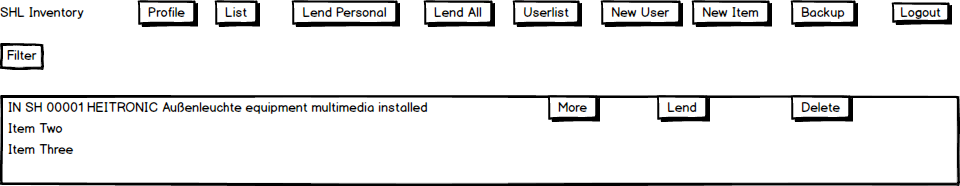
\includegraphics[scale=0.3]{content/pictures/MockUp.png}
	% bosch_iot_poll.png: 0x0 pixel, 300dpi, 0.00x0.00 cm, bb=
	\caption{MockUp von Items-Tabelle}
	\label{fig:mockup}
\end{figure}


Ist das Storytelling abgeschlossen und die möglichen Fehler beseitigt wurden, so kann das MockUp beginnen. Beim MockUp, in der Webentwicklung, wird das Layout schemenhaft mit Bleistift und Papier erzeugt. Dabei tritt das Designe stark in den Hintergrund, es ist in erster Linie wichtig, das verstanden wird, wie die Anwendung mit Button, Formulare und weiteren Elemente funktionieren. Das MockUp macht es später für die Entwicklung leichter, wenn es um die Umsetzung der Webanwendung geht. Bei der Erstellung des MockUp's hat man die Programmierung immer im Hinterkopf. Dabei wird überlegt wie Elemente angelegt werden.

\newpage

\section{User Experience}
\acf{UX} wurde häufiger in dieser Ausarbeitung verwendet und wurde noch nicht genauer erklärt. Das geschieht nun. Bei der \acl{UX}, auf deutsch \textit{Benutzererfahrung}, spricht man davon, wie der Benutzer mit Software Umgeht. Dabei greift man auf eigene Erfahrungen zurück, es gibt allerdings auch Werkzeuge um eine gute Benutzbarkeit zu messen. \autocite{Moser.2012} Dazu gehört Beispielsweise das Storyboard, welches mit hilfe des Storytelling Geschichten mit Bilder erzählt. Für dieses Projekt wurde auf kurze Wege geachtet, das der User die Maus nicht allzu sehr die Maus bewegen. Auch wird dem User durch das Designe gezeigt was klickbar ist und was nicht. Unbewusst wird er eine Gruppierung vornehmen. So sind Buttons, mit welchen etwas erzeugt wird, wie \textit{New Item}, \textit{New User} und \textit{Backup}, mit einem anderen Hintergrund und einer Umrandung versehen. 

\begin{figure}[bh]
	\centering
	
\includegraphics[scale=0.3]{content/pictures/gruppierung.png}
	% bosch_iot_poll.png: 0x0 pixel, 300dpi, 0.00x0.00 cm, bb=
	\caption{Button Gruppierung}
	\label{fig:gruppierung}
\end{figure}

%\subsection{Fitts Gesetze}

\section{Frameworks}
Wenn man Framework in die deutsche Sprache übersetzt, so erhält man das Wort Rahmengerüst. In der Softwareentwicklung spricht man von solchen Frameworks bei Programmierstruckturen, welche den Entwickler unterstützen. Dabei handelt es sich nicht um eine fertige Software. Es handelt sich um bewährte Programmierstruckturen, welche dem Entwickler die Arbeit abnehmen. So werden bekannte Entwurfsmuster übernommen werden. Auch aufwendige Funktionen sind in Frameworks schon häufig implementiert. Der Entwickler muss sich nicht mehr aufwendig um eine Datenverbindung kümmern oder kann komplizierte Animationen mit wenigen Zeilen Code erstellen. Eine wichtige Aufgabe während der Softwareentwicklung ist das Testen. Hier werden mithilfe des Frarmeworks Tests geschrieben, mit welchen kontrolliert werden kann, ob die Software korrekt funktioniert. Frameworks kommen meistens in der Objektorientierung zum Einsatz. Ihre Einsatzgebiete können vielseitig sein. Man findet sie in der Softwareentwicklung, bei der Entwicklung von Spielen und in der Webentwicklung.

\section{Wahl der Frameworks}
\label{chapter:frameworkchoice}
Bei der Wahl der Frameworks wurde analysiert welches sicher läuft, eine große und aktive Community hat, wenig Einrichtungen erfordern und in welchen die meisten Erfahrungen schon vorhanden sind. Bei der Wahl des Frontend-Frameworks fiel die Wahl schon früh auf Angular. Es wird bis heute noch von Google weiterentwickelt und hat eine sehr große Community. Die Erfahrungen in JavaScript sind ebenfalls vorhanden und die meiste Einrichtungen sind schon vorhanden oder werden von dem Framework selbst übernommen. Bei der Wahl des Backend-Frameworks war die Wahl nicht so einfach. Es standen Tomcat, ein Java-Framework und Laravel, ein \acs{PHP}-Framework, zur Auswahl. Es wurde Laravel gewählt, da es von sich aus viele Aufgaben, wie Sicherheit, Datenbankverwaltung oder Benutzerverwaltung mit Login-System übernimmt. \acs{PHP} und MySQL waren auf dem Server installiert. Für Tomcat hätte eine separate Installation erfolgen müssen.
